
% Using HBase for data and metadata
\sys\ was incepted with the  goal of adding transactional access on top of HBase,
though it can work with any strongly consistent key-value store that provides multi-versioning with version 
manipulation and atomic \emph{putIfAbsent} insertions as we now describe.

The underlying data store offers \emph{persistence} (using a write-ahead-log), \emph{scalability} (via sharding),  and \emph{high availability} (via replication) of the data plane, relieving \sys\ to manage only the transaction control plane.
\sys\ further relies on the underlying data store 
for fault-tolerant and persistent storage of transaction-related metadata.
This metadata includes a dedicated table that holds a single record per committing transaction, and 
in addition, per-row metadata for items accessed transactionally.
The \sys\ architecture is illustrated in Figure~\ref{fig:Omid_Architecture}.

\begin{figure}[t]
\centerline{
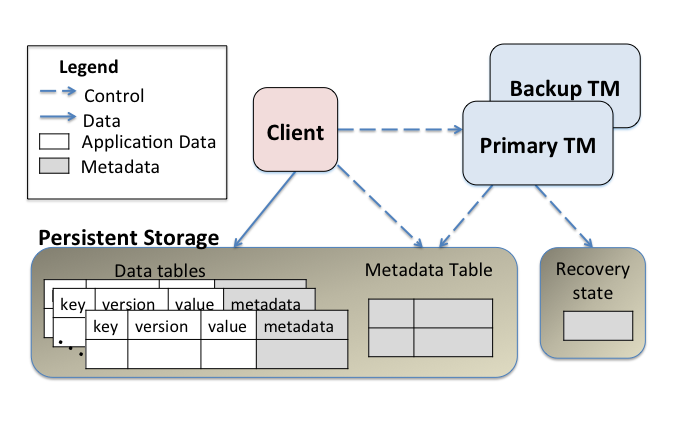
\includegraphics[width = 0.95\columnwidth]{OmidComponents.png}
}
\caption{{\bf \sys\ architecture}. Clients manipulate data that resides in data tables in the underlying multi-versioned persistent data store (for example, HBase) and use the TM in the control path for conflict detection. Only the primary TM is active, and the backup is in hot standby mode. The TM maintains persistent metadata in the data store as well as separately managed recovery state (for example, using Zookeeper).}
\label{fig:Omid_Architecture}
\end{figure}


% MV
\sys\ leverages  \emph{multi-versioning}  in the underlying key-value store in order to allow transactions to read consistent snapshots of changing data as needed for snapshot isolation. The store's API allows users to manipulate versions explicitly. It supports atomic {\em put(key, val, ver)}  and  {\em putIfAbsent(key, val, ver)} operations for updating or inserting a new  item with a specific version, and an atomic {\em get(key, ver)} operation for retrieving the item's value with highest version not exceeding \emph{ver}.
Specifically, when the item associated with an existing key is overwritten, the new version (holding the key, its new value, and a new version number)  is created, while the previous version persists. 
An old version might be required as long as there is some active transaction that had begun before the transaction that overwrote this version has committed. Though this may take a while, overwritten versions eventually become obsolete. 
A cleaning process, (in HBase, implemented as a coprocessor~\cite{hbase-coproc}),
%\footnote{\small{\url{https://blogs.apache.org/hbase/entry/coprocessor_introduction}}}) 
frees up the disk space taken up by obsolete versions. 


% TM  
The transaction control plane is implemented by a centralized transaction manager.
%, backed by persistent storage in the underlying data store. 
The TM has three roles: (i) \emph{version (timestamp) allocation} for each transaction; (ii) \emph{conflict detection} in order to determine which transactions may commit; 
and (iii) \emph{persistent logging of the commits}.
The TM provides high availability via a primary-backup approach--- if the primary TM becomes unresponsive, then the backup becomes the new primary and takes over. 
This design offers durability and high availability; it further facilitates scalability of storage and compute resources separately -- 
metadata storage access scales out on the underlying distributed data store, whereas 
conflict management is done entirely in RAM, and scales up on a shared-memory multi-core server. 

% TM conflict detection
Conflict detection
is lightweight and can be performed at a high throughput -- at least an order of magnitude faster than the transaction 
processing rates the network can sustain.
For example, with 
eight threads, it can handle 
%typical workload at the rate of 
five million transactions per second.
%, with an average of two data items accessed per transaction. 
To reduce the communication cost and RAM footprint of the TM, we use approximate conflict detection, which is 
based on hashes rather than  full keys, and also represents some information in aggregate form. 
Although this may lead to false aborts, the abort rates witnessed both in production and 
in microbenchmarks are negligible.

% We describe the commit protocol and conflict detection mechanism in Section~\ref{sec:protocol}.

% HA
Our high availability solution tolerates ``false'' fail-overs, where a new primary replaces one that is simply slow,
(for example, due to a garbage collection stall), leading to a period with two active primaries.
Synchronization between the two  is based on  shared persistent metadata storage, 
and induces overhead only in rare cases when more than one TM acts as primary.
\sys\ uses time-based leases in order to minimize potential overlap among primaries. 
The implementation employs Apache Zookeeper~\cite{zookeeper}
%\footnote{\small{\url{http://zookeeper.apache.org}.}} 
for lease management and synchronization between primary and backup. 
%This mechanism is described in detail in Section~\ref{sec:ha}.
